
\begin{figure}[t]
    \centering
    % \hspace{-10mm}
    \subfigure[SST-2]{
        \begin{minipage}[t]{0.5\linewidth}
        \centering
        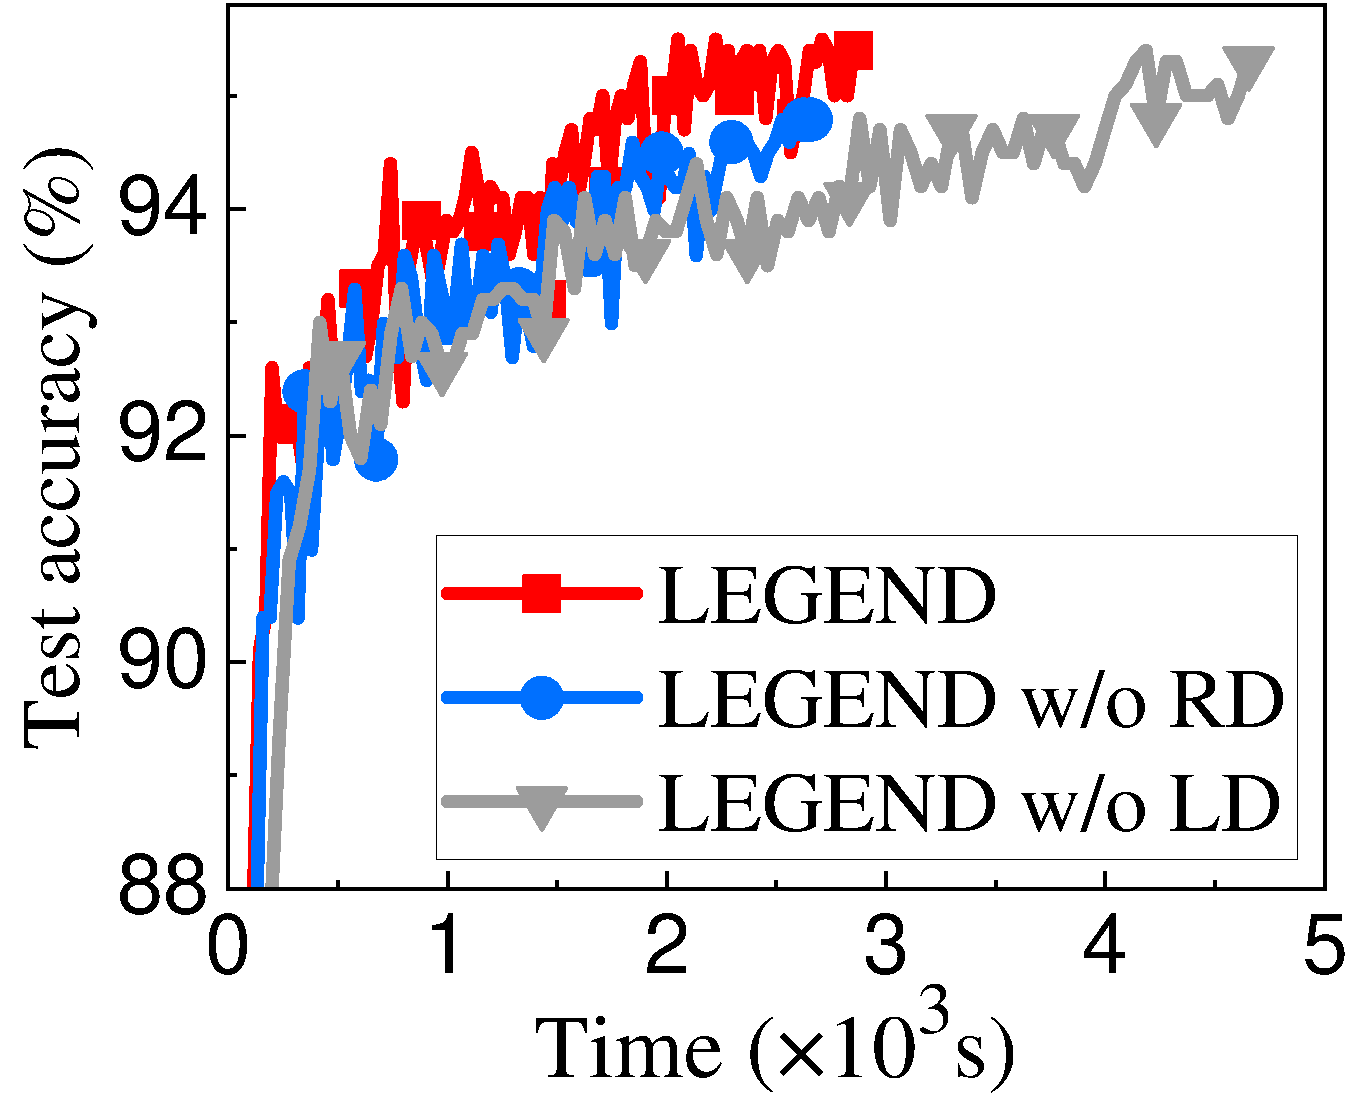
\includegraphics[width=1.6in]{figs/ablation-module-sst2-time2acc.pdf}
        \end{minipage}%
        \label{ablation-rank-time2acc-sst2}
    }%
    \subfigure[QNLI]{
        \begin{minipage}[t]{0.5\linewidth}
        \centering
        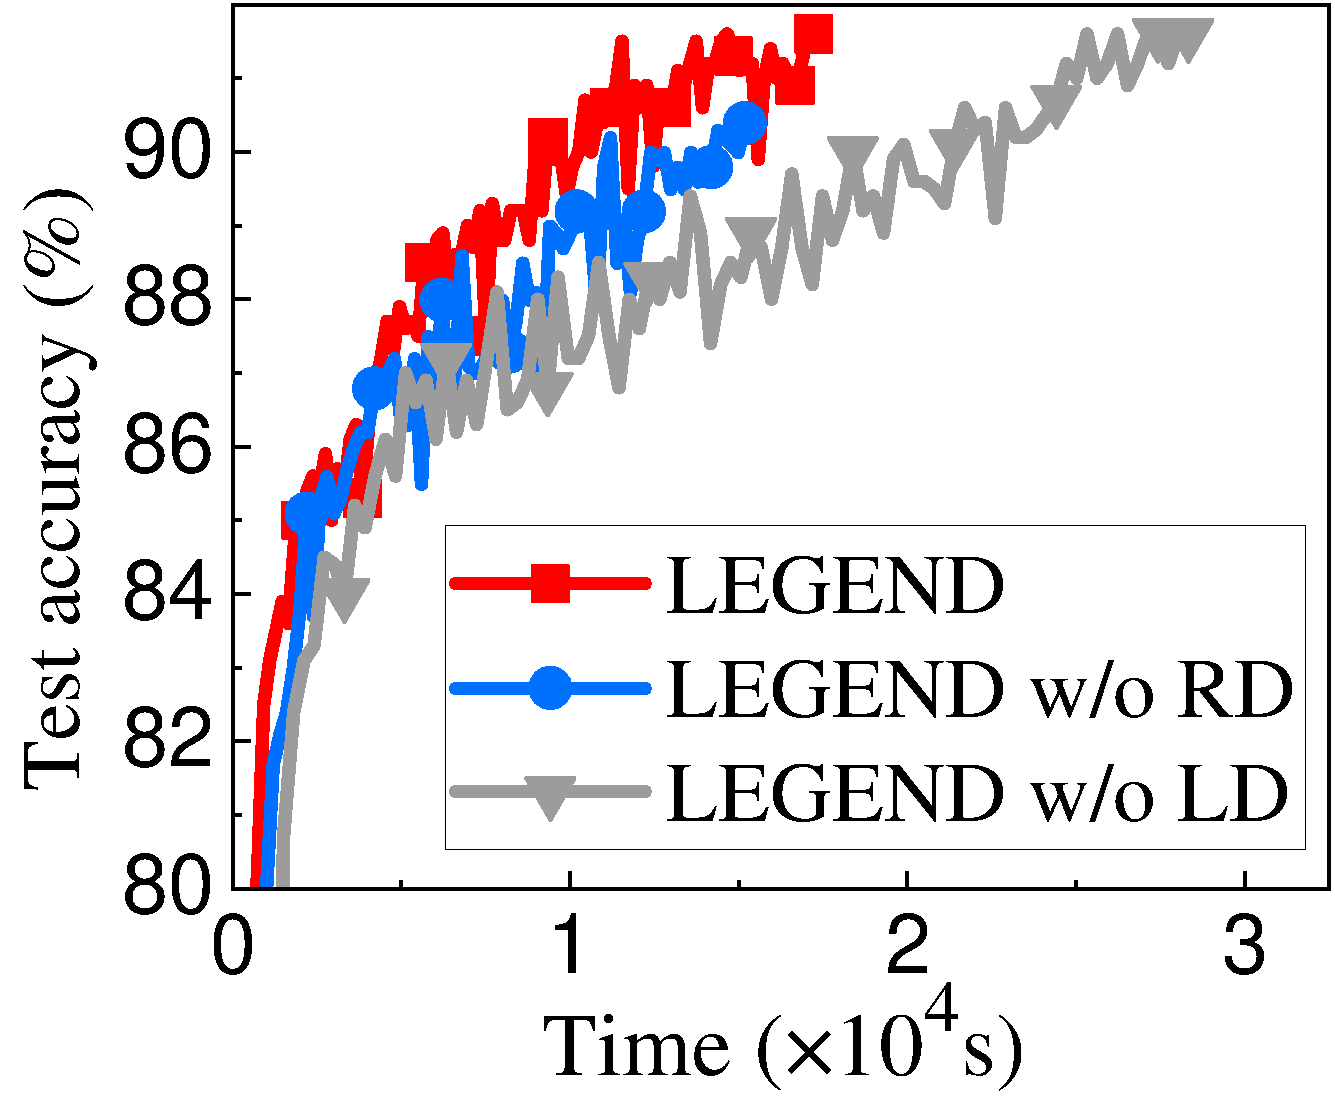
\includegraphics[width=1.6in]{figs/ablation-module-qnli-time2acc.pdf}
        % 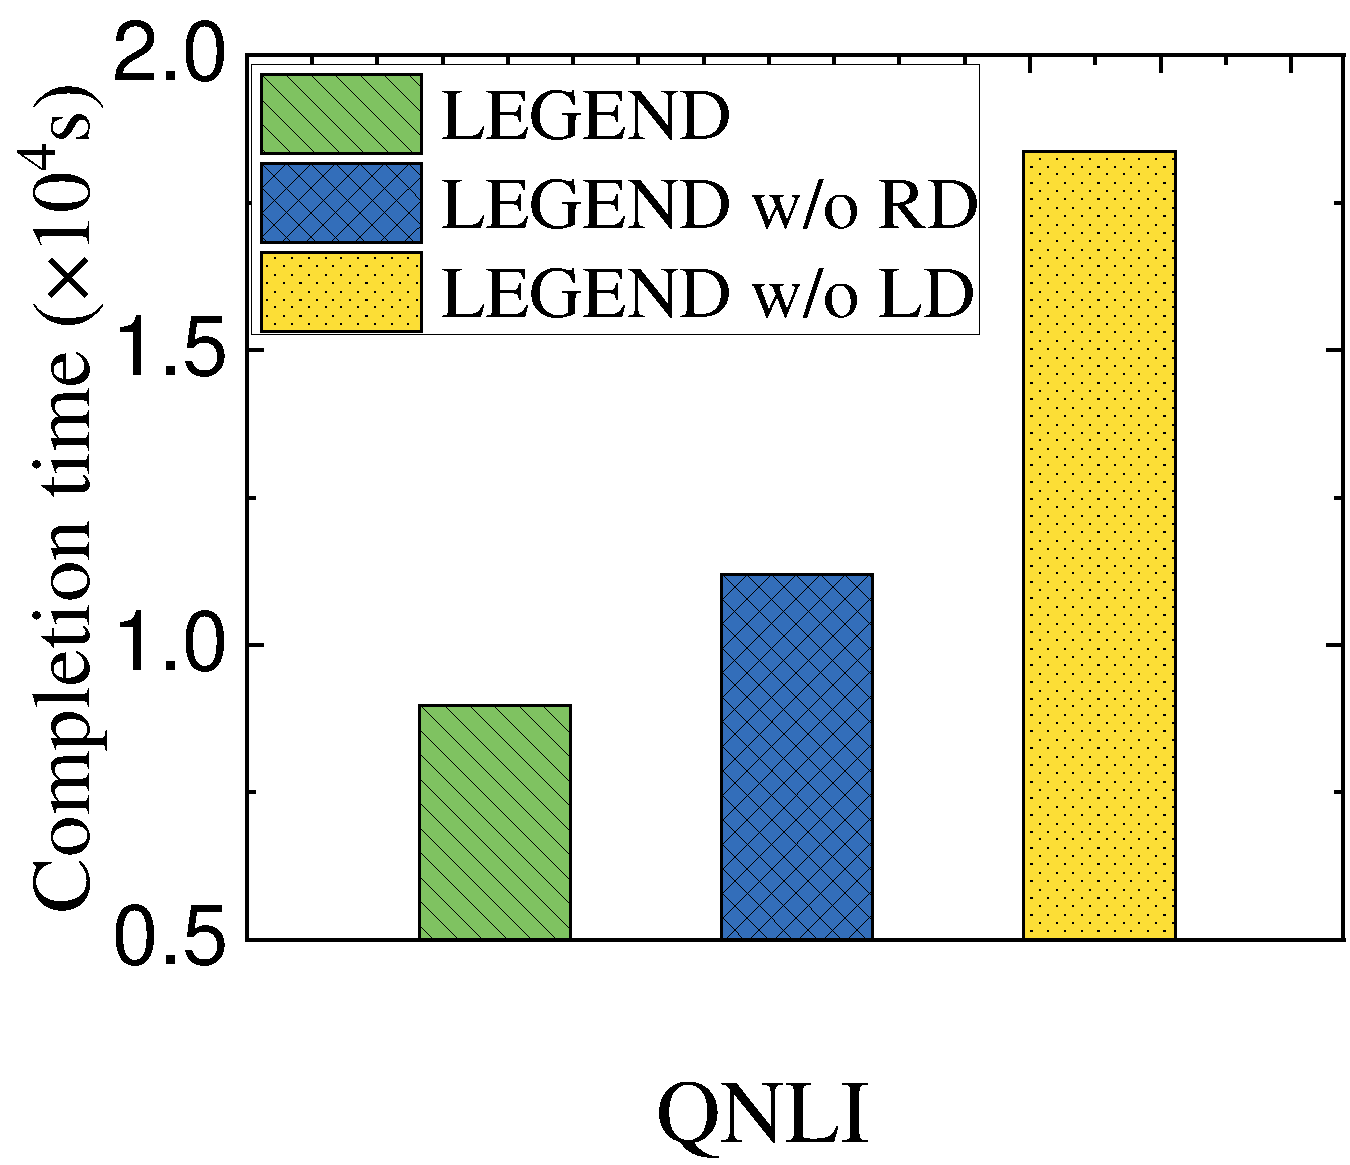
\includegraphics[width=1.5in]{figs/ablation-module-qnli-completion-time.pdf}
        \end{minipage}%
        \label{ablation-rank-time2acc-qnli}
    }%
    \centering
    \vspace{-0.35cm}
    \caption{Effect of LoRA depth and rank distribution.}
    \label{ablation}
    \vspace{-0.4cm}
\end{figure}

\vspace{-0.2cm}
\textbf{Natural Language Processing.}
The development of modern natural language processing (NLP) traces back to the introduction of the transformer architecture by Vaswani \etal in 2017 \cite{vaswani2017attention}. 
Upon transformer architecture, groundbreaking language models, such as BERT \cite{devlin2018bert}, GPT-2 \cite{radford2019language}, and more recently Llama \cite{touvron2023llama}, have achieved state-of-the-art results across various NLP tasks. 
Specifically, the language model (LM) is first pre-trained on a large corpus to learn general features and patterns. 
Subsequently, the LM is further trained on domain-specific data generated on devices to enhance the model performance for a specific task \cite{devlin2018bert, brown2020language}. 
However, due to data privacy, it is impractical to collect enough data from the devices for centralized fine-tuning \cite{mcmahan2017communication, lin2021fednlp}. 

\textbf{Federated Fine-Tuning.} 
To fully utilize the massive data on devices, federated fine-tuning (FedFT) has been proposed to perform fine-tuning in a distributed manner \cite{lin2021fednlp}.
% In the typical FedFT framework, \eg, FedNLP \cite{lin2021fednlp}, under the coordination of the parameters server (PS), participating devices periodically fine-tune the LMs locally without exposing their raw data, and push the entire LMs to the PS for global aggregation.
% The fine-tuning procedure is repeated for multiple rounds until the model convergence. 
However, the high resource costs associated with FedFT pose significant challenges to its practical implementation.
Modern FedFT utilizes parameter-efficient fine-tuning (PEFT) methods, such as Adapter \cite{houlsby2019parameter, cai2022fedadapter}, prompt-tuning \cite{lester2021power, zhao2023fedprompt}, to reduce on-device resources costs. 
For example, Cai \etal \cite{cai2022fedadapter} first apply Adapter in FedFT and propose FedAdapter, which dynamically searches for the optimal Adapter structure to improve the fine-tuning efficiency.
However, due to the intrinsic property of Adapter, the fine-tuned Adapter-based LM inevitably brings additional inference latency, potentially resulting in up to a 30\% latency increase \cite{hu2021lora, liao2023parameter, li2024caraserve}, which is often unacceptable in practical applications. 
Upon prompt-tuning, Zhao \etal \cite{zhao2023fedprompt} propose FedPrompt to realize communication-efficient and privacy-preserving fine-tuning in federated setting.
Nevertheless, prompt-tuning unavoidably occupies a portion of the model's input length, consequently diminishing the usable input space and extra inference latency.


\textbf{Low-Rank Adaptation.}
To mitigate the disadvantages of the aforementioned PEFT methods, Hu \etal \cite{hu2021lora} propose low-rank adaptation (LoRA), which adds trainable rank decomposition matrices to each transformer layer of the LM while freezing the pre-trained weights of the LM to improve fine-tuning efficiency. 
LoRA achieves comparable performance of fully fine-tuning while introducing no additional inference latency, and has been widely adopted.
For instance, Dettmers \etal \cite{dettmers2024qlora} propose QLoRA, which is an efficient fine-tuning method based on model quantization, significantly reducing the memory requirement.
Chen \etal \cite{chen2023longlora} propose LongLoRA, which is an efficient fine-tuning approach to extend the context sizes of the LM with limited cost.



% FedBitFit \cite{zhang2023fedpetuning} only updates LM biases, leading to limited performance on larger datasets. FedPrompt \cite{zhao2023fedprompt} uses Prompt-tuning, which increases inference latency and limits usable sequence length. 
% Then, Hu \etal propose low-rank adaptation (LoRA) for fine-tuning LMs without extra latency.
% For example, Cai \etal \cite{cai2022fedadapter} first introduce Adapter into FedNLP and propose FedAdapter and Zhang \etal validate the effectiveness of Adapter, BitFit, Prompt-tuning, and LoRA techniques in FedNLP.
% Although the PEFT can save massive computing and communication overhead, the inherent shortcomings of PEFT remain unsolved, leading to new problems for fine-tuning LMs on resource-constraint and heterogeneous devices.
% For example, FedAdapter\cite{cai2022fedadapter} does not solve the inference latency problem caused by the Adapter, resulting in an additional inference latency of up to 30\% \cite{hu2021lora}.
% FedBitFit\cite{zhang2023fedpetuning} only updates the bias of LMs, resulting in limited fine-tuning performance and degrading significantly compared to full fine-tuning when applied to larger datasets. 
% In addition, FedPrompt \cite{zhao2023fedprompt} is based on Prompt-tuning, which trains a continuous prompt that is prepended to inputs for each task. 
% Prompt-tuning leads to longer inference latency, takes up available input length, and limits the real usable sequence length. 
% On the contrary, LoRA achieves satisfactory performance without incurring extra inference latency. 



\textbf{FedFT with LoRA.}
LoRA is naturally incorporated into FedFT to reduce resource costs.
% while achieving comparable performance. 
For example, Zhang \etal \cite{zhang2023fedpetuning} propose FedLoRA and verify the efficiency of LoRA in the context of FedFT through extensive experiments.
Upon FedLoRA, Cho \etal \cite{cho2023heterogeneous} propose HetLoRA, in which each device adds LoRA layers to all transformer layers with a diverse and appropriate LoRA rank to deal with system heterogeneity.
However, due to the rank mismatch of all LoRA layers on different devices, it is difficult to aggregate these layers, resulting in poor fine-tuning performance.
In conclusion, existing works simply add LoRA layers with the uniform rank distribution for all transformer layers, which still requires substantial computing and communication resources, resulting in slow fine-tuning speeds on weak devices. 
Moreover, system heterogeneity further leads to low fine-tuning efficiency or poor fine-tuning performance \cite{kim2021autofl, luo2022tackling}.
They do not address the challenges of resource constraints and system heterogeneity.
% In other words, in the context of FedFT, existing works still face significant limitations, as they fail to achieve both high accuracy and fast convergence.
% This is especially evident with resource-constrained and heterogeneous devices, where these methods fail to effectively address the above challenges.
% On the contrary, LEGEND generates reasonable rank distribution to enhance the fine-tuning performance and assigns different LoRA depths for heterogeneous devices to improve fine-tuning efficiency, effectively addressing the aforementioned challenges while saving resource costs.
\vspace{-0.2cm}


